Proceso por el cual un medio absorbe energía de una onda que lo atraviesa, reduciendo su amplitud y eventualmente su intensidad. Ocurre cuando la energía de la onda se transforma en otra forma de energía, generalmente calor, dentro del material.

Esto se puede observar en el espectro de absorción de los hojas. La clorofila no absorbe toda la luz solar uniformemente. Las moléulas de clorofila preferentemente absorben la luz roja (con picos de aborción de $600-700 nm$ del \EspectroElectromagnetico) y azul (con picos de aborción de $400-500 nm$) para usar en la fotosíntesis, pero mucho menos en la luz verde (picos de absorción de $500-600 nm$) es absorbida y por tanto una gran cantidad es reflejada\cite{doncontrolhojas}.

\begin{figure}[H]
  \centering
  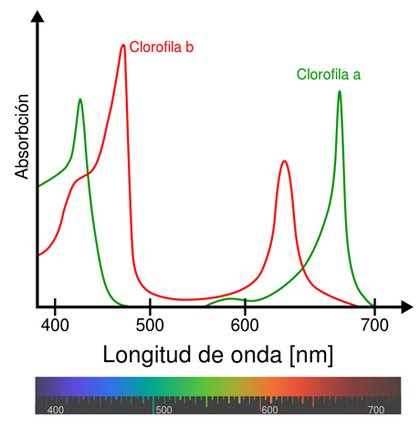
\includegraphics[scale=0.6]{imagenes/absorcion_hojas.png}
  \caption{Espectro de absorción de las hojas\cite{doncontrolhojas}}
\end{figure}
